%&latex
\documentclass{report}
\usepackage{graphicx} 
\usepackage{wrapfig}
\usepackage{enumitem}
\usepackage{amsmath}
%+Make Index
\usepackage{makeidx}
\makeindex
%-Make Index

\begin{document}

%+Title
\title{\Huge\bf Export of Modelica models to the ProMoVis environment}
\author{Jesper Moberg}
\date{\today}
\maketitle
%-Title

%+Contents
\tableofcontents
%-Contents

\chapter{DRAFT}
\section{questions}
\begin{itemize}
\item The constant vector, g, how should that one be treated if it is non-zero( how is it treated in the modelica model)?
\item how do we design so that you can rework your modelica model, but still keep the scenario layouts that the user has created.
\item check all "FIXMES" since there are some question embedded in these to.

\end{itemize}
\section{Example model}
When explaining we sometimes reference this model to clarify stuff, fixme
\newpage




%The export tool makes the following initial assumptions about the Modelica model before linearizing it:
%\begin{itemize}
%\item The model is, at its intendened working point at time 0. 
%\end{itemize}
\chapter{Structure of the export tool}

\section{General structure}
To make the details of the export tool easier to grasp, the following chapter focuses on describing the structure and phases of the export tool, leaving the details out until subsequent chapters.\\\newline
\setlength\fboxsep{0pt}
\setlength\fboxrule{0.5pt}
\fbox{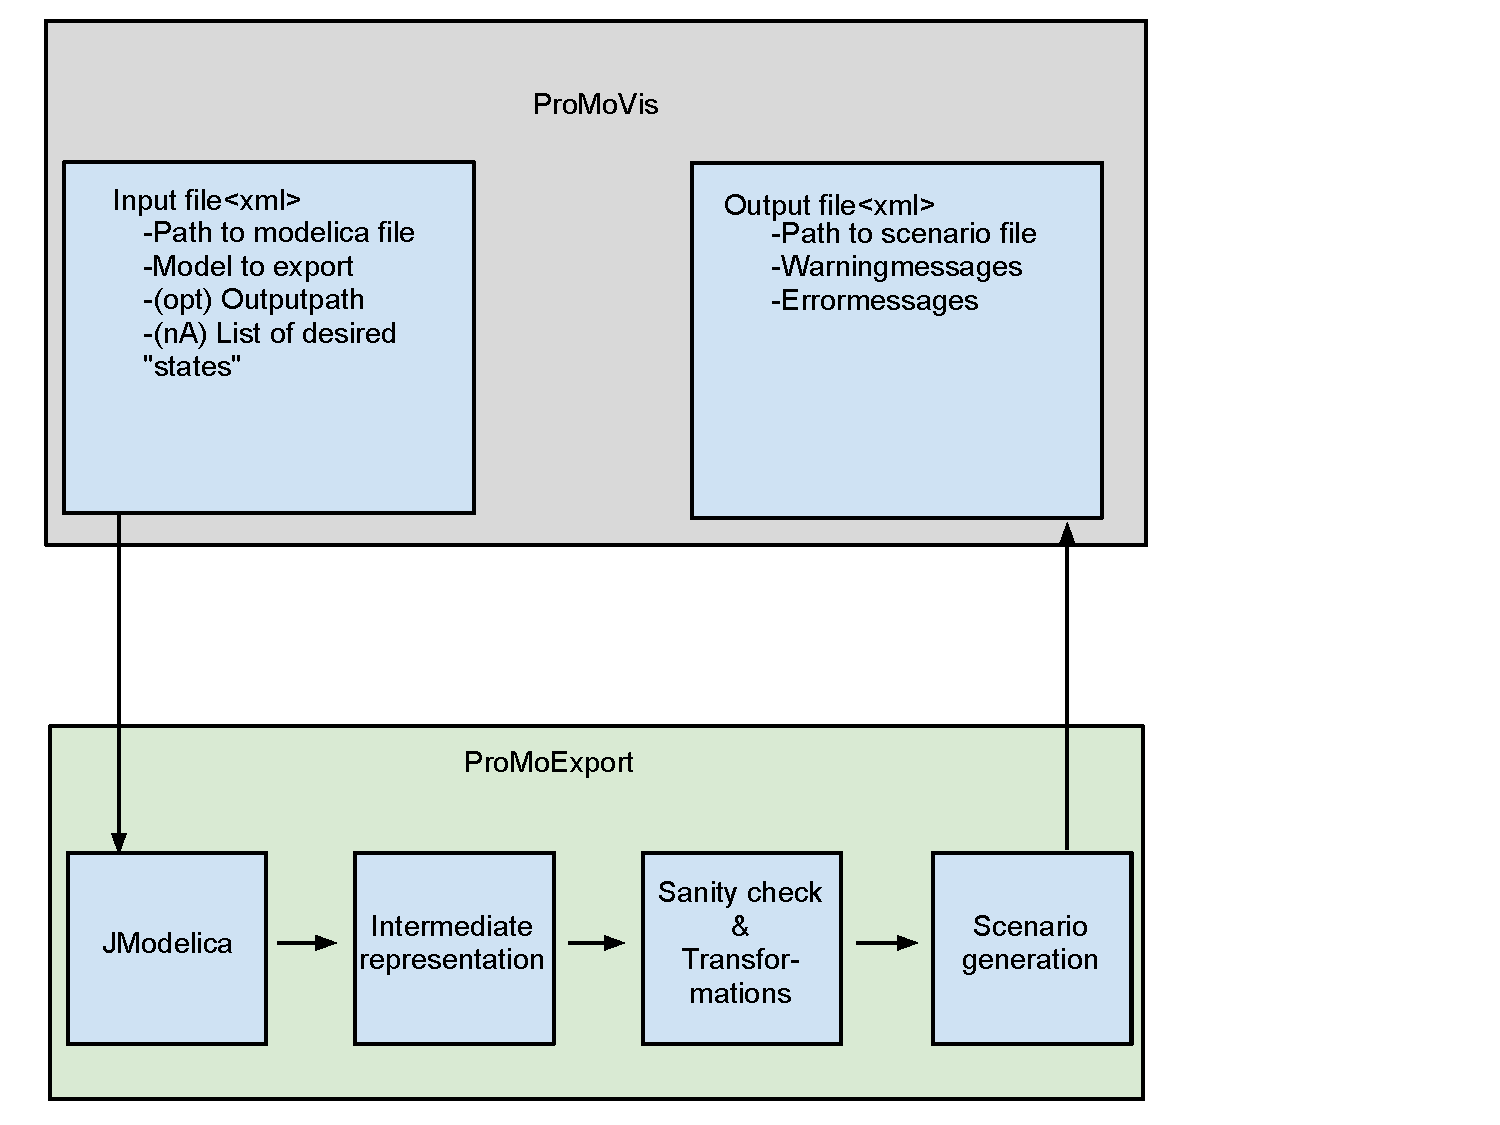
\includegraphics[scale=0.5,bb=0 0 215mm 194mm] {./pictures/frontend.pdf}}\\\newline There are two ways to run the export tool where one, indicated in the picture above, is through passing it an XML file containing parameters for the export, the other one is through importing the (FIXME)module into a python environment, and run each of the phases manually. Where the first is intended to be used when interfacing with other software(e.g. ProMoVis) while the later is intended to be used when developing the tool or when a users needs to do some additional manipulation of the compiled Modelica model before exporting it to ProMoVis.  \\\newline
The export to ProMoVis is divided into four distinct phases:
\begin{itemize}
\item \textit{JModelica}, the JModelica phase is where you compile the original Modelica model, linearize it and extract the information from the linear model.
\item \textit{Intermediate representation}, is the phase where the export tool, from the linear model, extract each of the states and their relations to other states, disturbances and inputs. Here the initial types for ProMoVis is indicated, so that modeled disturbances are "Disturbance variables", inputs are "Control variables" and all states are set to be "Internal Variables".
\item \textit{Sanity check \& Transformations}, is where the export tool do some checks on the model, and eventually generates warnings and errors regarding the linear model. This is also where it, if the user has defined them changes, the type of selected states, to be "Measured variables". \newline \textit{Note! This is for version 0.1, later versions might merge the transfer functions of states that are not of interest for the user.}
\item \textit{Scenario generation}, the last phases, creates the ProMoVis specific represenation of the model. It is also responsible for creating the layout of the ProMoVis model. In version 0.1 this can not be set by the user, instead it will try to achieve a circular model as shown in the following figure:  


\setlength\fboxsep{0pt}
\setlength\fboxrule{0.5pt}
\fbox{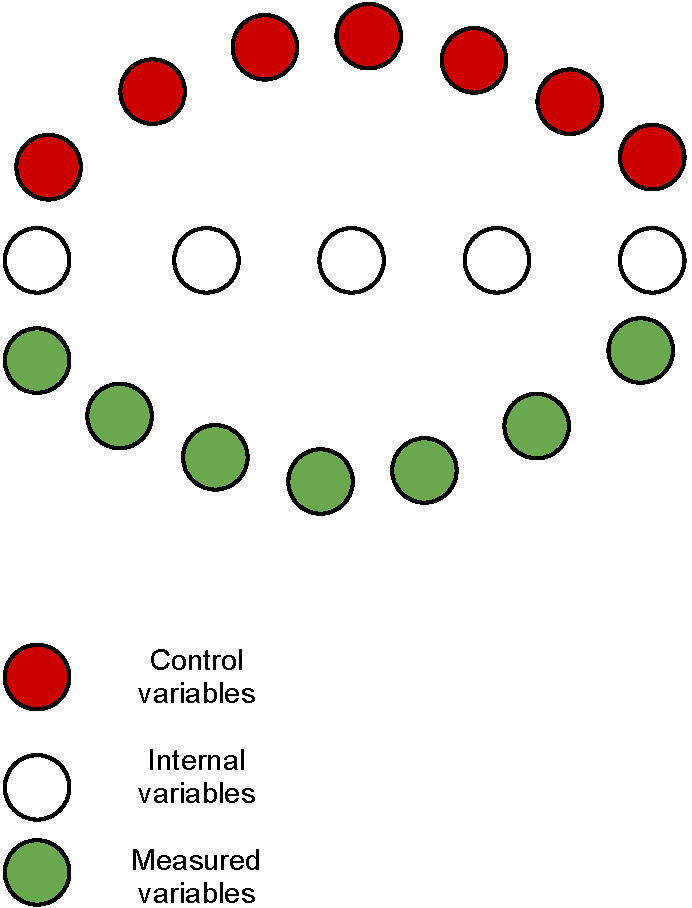
\includegraphics[scale=0.3,bb=0 0 118mm 154mm] {./pictures/layout.pdf}}\\\newline
Through this layout, the inside of the circle may become very cluttered, still the user should be able to see the measured and control variables from at the boundraries of the circle.\\\newline\\\newline 
\end{itemize}
Although, in version 0.1, there is no user interaction in between the phases, the export-tool is designed in such a way that, if it becomes necessary, one can add interactivity in between each of the phases. But for version 0.1 the only way to affect the output is through the parameter file passed as input to the tool.


\subsection{Intended workflow V.0.1}
In version 0.1, there is/was FIXME little integration between the tools. The user creates his model in an arbitrary Modelica environment and configure its initial values so that they correspond to the desired working points.
\\\newline



\setlength\fboxsep{0pt}
\setlength\fboxrule{0.5pt}
\fbox{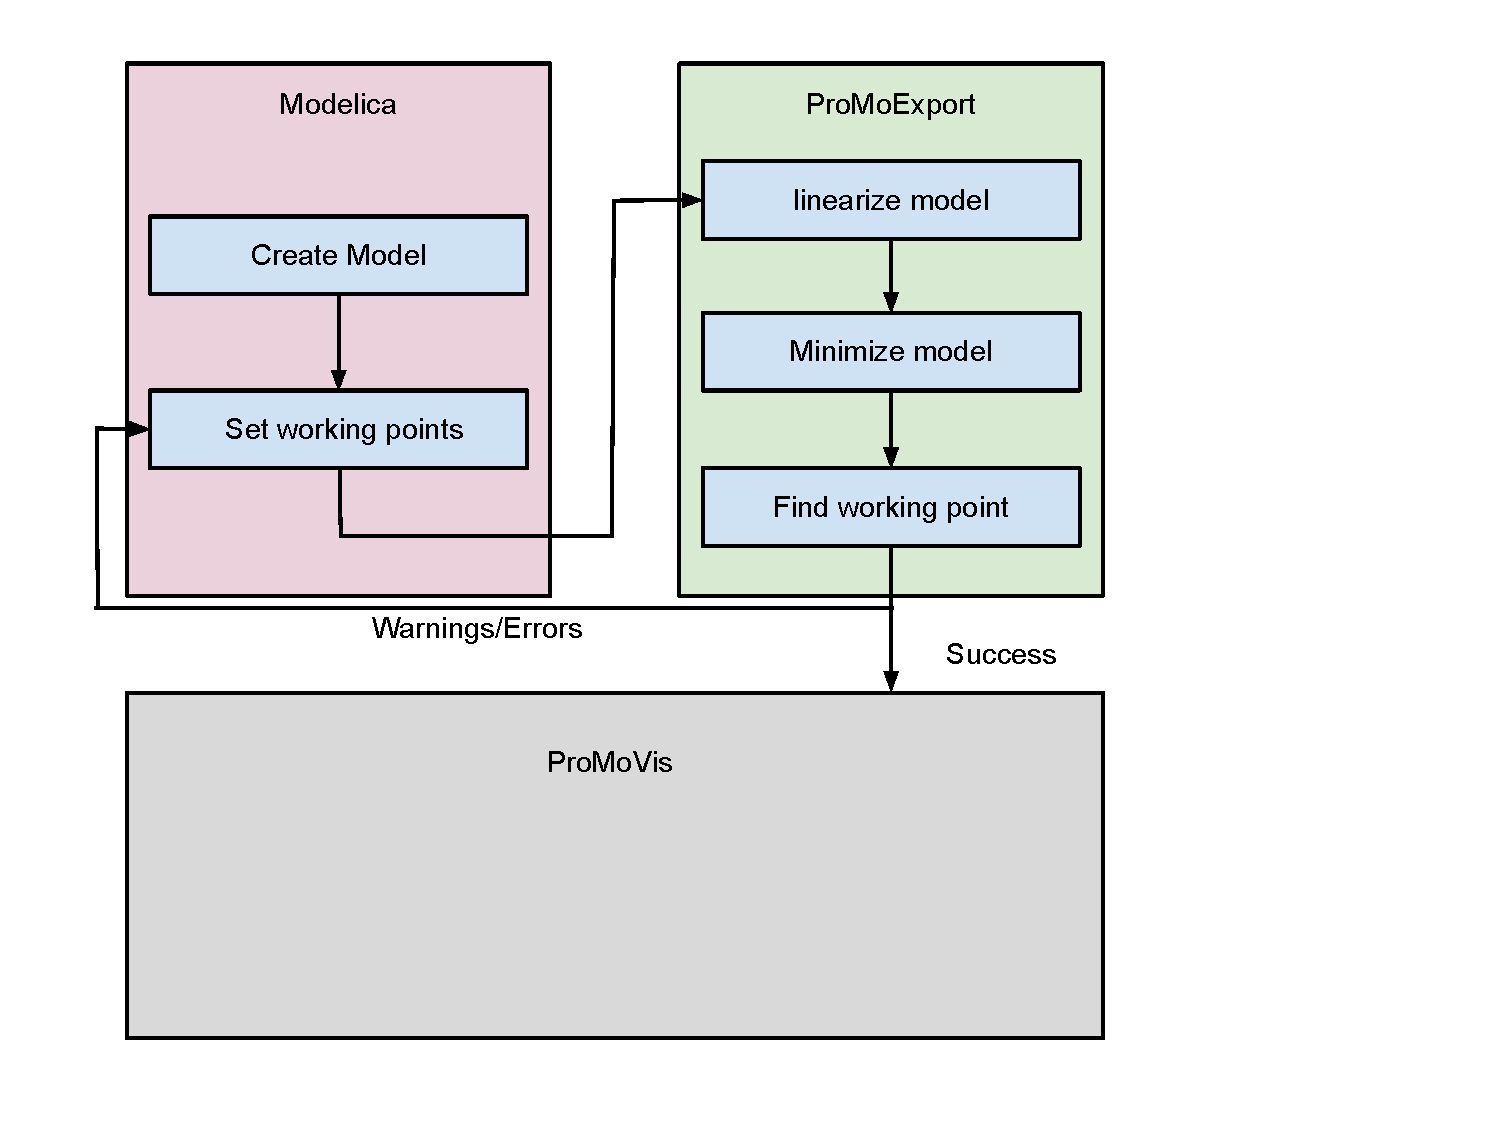
\includegraphics[scale=0.5,bb=0 0 215mm 194mm] {./pictures/workflow.pdf}}\\\newline

The idea here is that the user creates its model in modelica, run it through the export tool. If there is an error in the Modelica source file, the tool will generate an error and no scenario will be emitted. There is also the possibility that the tools generates a warning, when a warning is created a scenario is emitted but the user is strongly encourage to review its model and its selected working points.\\\newline
\section{JModelica}
\subsection{Background}
JModelica is an open-source Modelica environment  for compilation and simulation of Modelica models. Through its python front-end it provides an easy to use, still powerful way to perform complex tasks on compiled models while, at the same time, it is easy to interface it to other software. 

\subsection{How the export tool uses JModelica}
The JModelica environment is used to compile the Modelica models to JModelicas JMU representation \cite{PythonAPI}. This representation is internally represented as a, possibly nonlinear, DAE. This model, can through the JModelica environemnt be linearized and a model with the following represenation can be extracted:
\begin{equation}
E*dx = A*x + B*u + F*w + g
\end{equation}
Important to note is that the current version of JModelica\cite{JModelicaVer} does not separate between internal states and outputs. \\This represenation should be familiar, the x and dx vectors represents the states and outputs of the linearized system. The u vector represents declared inputs, w is modeled disturbances (FIXME are they modeled in modelica, or attached at simulation time cant find anything regarding this in modelica specification) and finally g is a constant bias.\\The linearization also outputs some useful information that we later use in the generation of ProMoVis scenarios:
\begin{itemize}
\item \textit{State names}, corresponding to the declared variable names from the original Modelica file.
\item \textit{Input names}, corresponding to the declared input names from the original Modelica file.
\item \textit{Working points} for the linear model \textit{dx0}, \textit{u0} and \textit{x0}. Which is used to provide feedback for the user regarding the (FIXME)sanity of the linearized model.
\end{itemize}

This information is  stored in a dictionary and used in subsequent steps to create the intermediate representation of the system.


\section{Intermediate representation}
\subsection{Structure}
\subsubsection{pmv\_scenario}
\begin{itemize}[label=]
\item \textbf{Members}
\end{itemize}
\begin{itemize}[label=\_\_]
\item\textit{(String,array)}matrix\_dict[]
\item\textit{(pmv\_variable)}variable\_arr[]

\end{itemize}
\begin{itemize}[label=]
\item \textbf{Methods}
\end{itemize}
\begin{itemize}[label=+]
\item\textit{(Self)}\_\_init\_\_(matrix\_dict[])
\item\textit{(String)}printMe()
\item\textit{(Element)}getAsXML()
\end{itemize}


\subsubsection{pmv\_variable}
\begin{itemize}[label=]
\item \textbf{Members}
\end{itemize}
\begin{itemize}[label=\_\_]
\item\textit{(String)}name]
\item\textit{(String,pmv\_tf)}state\_dict[]
\item\textit{(String,pmv\_tf)}input\_dict[]
%\item\textit{(String,pmv\_tf)}disturbance\_dict[]
\item\textit{(Int)}type
\item\textit{(String)}workingpoint

\end{itemize}
\begin{itemize}[label=]
\item \textbf{Methods}
\end{itemize}
\begin{itemize}[label=+]
\item\textit{(Self)}\_\_init\_\_(name,type,state\_dict[],disturbance\_dict[],input\_dict[])
\item\textit{(String)}printMe()
\item\textit{(Element)}getAsXMLVariable(doc,layout\_emitter)
\item\textit{(Element)}getAsXMLProcessModel(doc,layoutfactory)
\end{itemize}
These are just set to defaults atm, which are relevant to extract from the modelica model?:\\\newline
saturationMax\newline
saturationMin\newline
rangeSatMax\newline
rangeSatMin\newline
variance\newline
delay\newline
sample\_time\newline
rateLimiter\newline
variance\newline
delay\newline
resolution\newline


\subsubsection{pmv\_tf}
\begin{itemize}[label=]
\item \textbf{Members}
\end{itemize}
\begin{itemize}[label=\_\_]
\item\textit{(Double)}num[]
\item\textit{(Double)}den[]



\end{itemize}
\begin{itemize}[label=]
\item \textbf{Methods}
\end{itemize}
\begin{itemize}[label=+]
\item\textit{(Self)}\_\_init\_\_(num[],den[])
\item\textit{(String)}printMe()
\end{itemize}

\subsubsection{layout\_emitter}
\begin{itemize}[label=]
\item \textbf{Members}
\end{itemize}
\begin{itemize}[label=-]
\item\textit{no public members}




\end{itemize}
\begin{itemize}[label=]
\item \textbf{Methods}
\end{itemize}
\begin{itemize}[label=+]
\item\textit{(Self)}\_\_init\_\_((int)inputs,(int) measured, (int)internal, (int)disturbances)

\item\textit{(String)}getCord(pmv\_variable)
\end{itemize}
\subsection{Generation of the structure}

The generation of the internal structure is best illustrated with the following example.\\\newline
When the linearized model is extracted and we have all non-zero diagonal elements the system might be represented as:\\\newline
$
\begin{bmatrix} E_{11} & E_{12} \\ E_{21} & E_{22} \end{bmatrix} \left[ \begin{array}{c} x0' \\ x1' \end{array} \right]
= \begin{bmatrix} A_{11} & A_{12} \\ A_{21} & A_{22} \end{bmatrix} \times \left[ \begin{array}{c} x0 \\ x1 \end{array} \right] + \begin{bmatrix} B_{11} & B_{12} \\ B_{21} & B_{22} \end{bmatrix} \times \left[ \begin{array}{c} u0 \\ u1 \end{array} \right]$\\\newline
This can, in s-domain(FIXME is this the english expression) be written as:\\\newline
$
\begin{bmatrix} E_{11} & E_{12} \\ E_{21} & E_{22} \end{bmatrix}  \left[ \begin{array}{c} x0 \\ x1 \end{array} \right] \times s
= \begin{bmatrix} A_{11} & A_{12} \\ A_{21} & A_{22} \end{bmatrix} \times \left[ \begin{array}{c} x0 \\ x1 \end{array} \right] + \begin{bmatrix} B_{11} & B_{12} \\ B_{21} & B_{22} \end{bmatrix} \times \left[ \begin{array}{c} u0 \\ u1 \end{array} \right]$\\\newline
We might then, with the previously declared condition that all diagonal elements of the E-matrix are non-zero, reduce each of the rows to find a representation of the dependencies for each of the states. E.g. for row 0 and x0 the following steps are done:\\\newline$\begin{array}{rcl} E_{11}*x0*s  +E_{12}*x1*s=A_{11}*x0  +A_{12}*x1 +B_{11}*u0  +B_{12}*u1 \end{array}$\newline
$\begin{array}{rcl} (E_{11}*s-A_{11})*x0  =(A_{12}-E_{12}*s)*x1 +B_{11}*u0  +B_{12}*u1 \end{array}$\\\newline
Thus, for x0, we get the following relations(FIXME find a consistent naming):\\\newline
$\begin{array}{rcl} x0  = \frac{(A_{12}-E_{12}*s)}{(E_{11}*s-A_{11})}*x1 +\frac{B_{11}}{(E_{11}*s-A_{11})}*u0  +\frac{B_{12}}{(E_{11}*s-A_{11})}*u1 \end{array}$\\\newline
And we can represent this information, together with the information from the JModelica representation, as a pmv\_variable, that would look something like this:\\\newline
\setlength\fboxsep{0pt}
\setlength\fboxrule{0.5pt}
\fbox{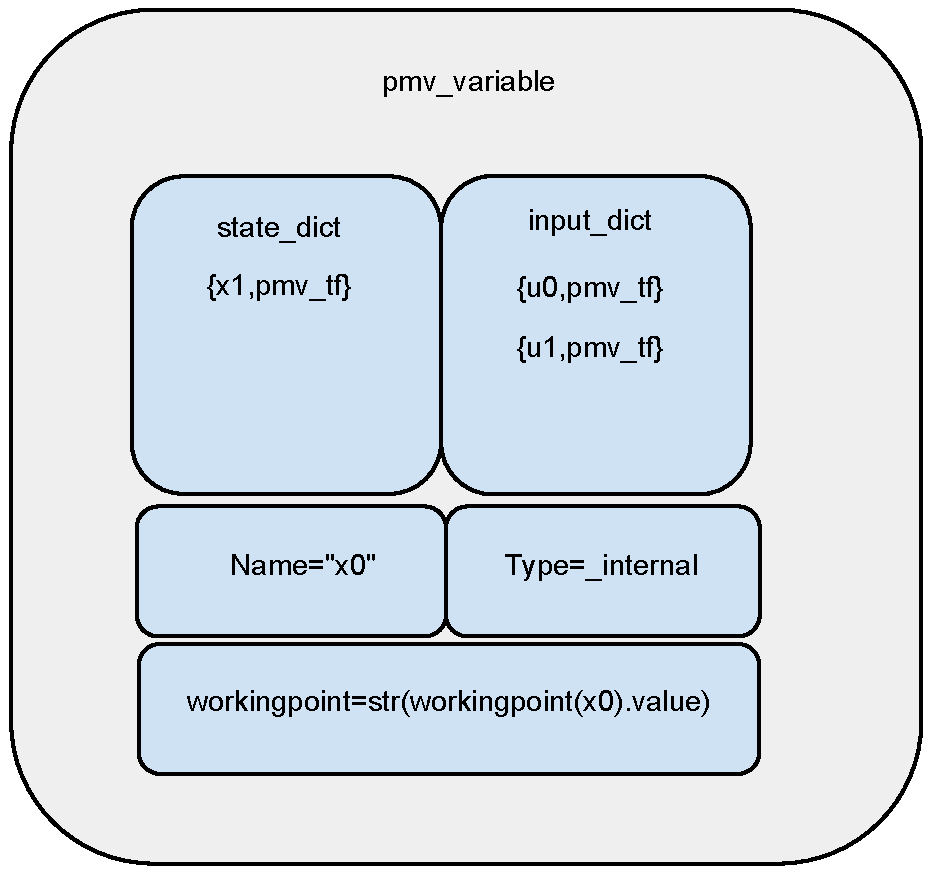
\includegraphics[scale=0.5,bb=0 0 159mm 150mm] {./pictures/pmv_var.pdf}}\\\newline

By now, it should be clear that a pmv\_variable is just a represenation of a state, together with all its dependencies (FIXME find a consistent naming).\\\newline A pmv scenario is built up by performing the described algebra for each of the models states and adding each of the resulting pmv\_variables to the variable\_arr.

\section{Sanity check and transformations}
Right now we only examine the derivatives at the linearization point, and if they are not "zero" we produce a warning.\\\newline Transformations:
In version 0.1, the only "transformation" that is performed, is that one only changes the "type" parameter, so that the ones specified by the user, is changed to "Measured" instead of "Internal".\\\newline
\textbf{TODO:} Get input, what do we need to examine, what rules/sensitivity should the warnings have?

\section{Scenario generation}
The scenario generation is done iteratively from the member, \textit{variable\_arr[]}, in the pmv\_scenario. The getAsXML() and getAsXMLProcessModel() is called for each of the variables. and inserted under the "Variables" and "ProcessModel" nodes respectively.\\\newline
Since the variable node also contains information regarding the visual representation of the systems a layout-emitter is a necessary argument to the getAsXMLProcessModel. The idea here is that the layout\_emitter should provide coordinates, additional images and other things regardning the visual representation. In v.0.1 it has only one constructer, taking as arguments, the amount of each of the variable types. It uses this information to calculate stepsizes and offsets so that it can create the circular structure described earlier.\\\newline Each of the calls to getAsXMLVariable, will call the getCord() method of the same instance of a layout\_emitter, which in turn will return the appropriate coordinates. Incrementing the "count" each time, so that the coordinates are moved.
\\\newline

(FIXME Questions to Johan?) Right now each of the pmv\_variables calls this to get coordinates, maybe this should be delegated to create the whole "NamedScenarioObject" node. Should one build it so that the layout emitter might create the images used in visualisation too? \\\newline

\chapter{Interfacing with the user/ other software}
Todo: Fix this after discussion with potential users.
%+Bibliography
\begin{thebibliography}{99}
\bibitem{PythonAPI} JModelica.org python api docs 
\bibitem{JModelicaVer} 1.7b2
\end{thebibliography}
%-Bibliography

%+MakeIndex
\printindex
%-MakeIndex


\end{document}


